\documentclass[12pt, a4paper]{article}

\usepackage{graphicx}

\begin{document}

\title{Notes on Axisymmetric Nozzle Design by Method of Characteristics}
\author{Hiromasa Kato}
\date{Feb. 16, 2017}
\maketitle

\section{2-dimensional Method of Characteristics}

\begin{eqnarray}
d(\theta + \nu) &=& 0~~~\mathrm{along}~C^-~\mathrm{characteristics} \\
d(\theta - \nu) &=& 0~~~\mathrm{along}~C^+~\mathrm{characteristics}
\end{eqnarray}
or
\begin{eqnarray}
\theta + \nu &=& K^- = \mathrm{const.}~~~\mathrm{along}~C^-~\mathrm{characteristics} \\
\theta - \nu &=& K^+ = \mathrm{const.}~~~\mathrm{along}~C^+~\mathrm{characteristics}
\end{eqnarray}
where $\theta$ is the flow angle in the $x$-$y$ plane and $\nu$ the Prandtl-Meyer function given by
\begin{equation}
\nu(M) = \sqrt{\frac{\gamma + 1}{\gamma - 1}} \tan^{-1}\sqrt{\frac{\gamma - 1}{\gamma + 1}\left(M^2 - 1\right)}
 - \tan^{-1}\sqrt{M^2 - 1}.
\end{equation}

\section{Method of Characteristics for Axisymmetric Flow}

\begin{figure}[!h]
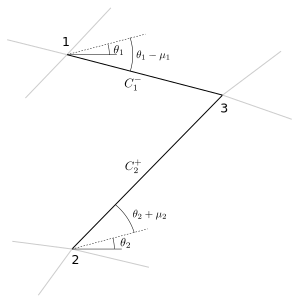
\includegraphics{InteriorPoint.pdf}
\end{figure}

Compatibility relations for axisymmetric flows in the cylindrical coordinate system ($x$-$r$) are given by\cite{anderson2004modern}
\begin{eqnarray}
d(\theta + \nu) &=& \frac{1}{\sqrt{M^2 - 1} - \cot\theta}\frac{dr}{r}~~~\mathrm{along}~C^-~\mathrm{characteristics} \\
d(\theta - \nu) &=& -\frac{1}{\sqrt{M^2 - 1} + \cot\theta}\frac{dr}{r}~~~\mathrm{along}~C^+~\mathrm{characteristics} 
\end{eqnarray}
An alternative formulation\cite{liepmann1957elements} is given, for example, as
\begin{eqnarray}
\frac{\partial}{\partial\xi}\left(\nu + \theta\right) &=& \sin\mu\frac{\sin\theta}{r} \\
\frac{\partial}{\partial\eta}\left(\nu - \theta\right) &=& \sin\mu\frac{\sin\theta}{r}
\end{eqnarray}
where $\xi$ and $\eta$ are the coordinate directions in the $C^+$ and $C^-$ characteristics, respectively.

\bibliography{bib}
\bibliographystyle{plain}

\end{document}
